 % This is the Reed College LaTeX thesis template. Most of the work
% for the document class was done by Sam Noble (SN), as well as this
% template. Later comments etc. by Ben Salzberg (BTS). Additional
% restructuring and APA support by Jess Youngberg (JY).
% Your comments and suggestions are more than welcome; please email
% them to cus@reed.edu
%
% See http://web.reed.edu/cis/help/latex.html for help. There are a
% great bunch of help pages there, with notes on
% getting started, bibtex, etc. Go there and read it if you're not
% already familiar with LaTeX.
%
% Any line that starts with a percent symbol is a comment.
% They won't show up in the document, and are useful for notes
% to yourself and explaining commands.
% Commenting also removes a line from the document;
% very handy for troubleshooting problems. -BTS

% As far as I know, this follows the requirements laid out in
% the 2002-2003 Senior Handbook. Ask a librarian to check the
% document before binding. -SN

%%
%% Preamble
%%
% \documentclass{<something>} must begin each LaTeX document
\documentclass[12pt,twoside]{reedthesis}
% Packages are extensions to the basic LaTeX functions. Whatever you
% want to typeset, there is probably a package out there for it.
% Chemistry (chemtex), screenplays, you name it.
% Check out CTAN to see: http://www.ctan.org/
%%
\usepackage{graphicx,latexsym}
\graphicspath{ {./figure/} }
\usepackage{amsmath}
\usepackage{amssymb,amsthm}
\usepackage{longtable,booktabs,setspace}
\usepackage{chemarr} %% Useful for one reaction arrow, useless if you're not a chem major
\usepackage[hyphens]{url}
% Added by CII
\usepackage{hyperref}
\usepackage{lmodern}
\usepackage{float}
\floatplacement{figure}{H}
% End of CII addition
\usepackage{rotating}


\usepackage{makeidx}
\makeindex


% Next line commented out by CII
%%% \usepackage{natbib}
% Comment out the natbib line above and uncomment the following two lines to use the new
% biblatex-chicago style, for Chicago A. Also make some changes at the end where the
% bibliography is included.
%\usepackage{biblatex-chicago}
%\bibliography{thesis}


% Added by CII (Thanks, Hadley!)
% Use ref for internal links
\renewcommand{\hyperref}[2][???]{\autoref{#1}}
\def\chapterautorefname{Chapter}
\def\sectionautorefname{Section}
\def\subsectionautorefname{Subsection}
% End of CII addition

% Added by CII
\usepackage{caption}
\captionsetup{width=5in}
% End of CII addition

% \usepackage{times} % other fonts are available like times, bookman, charter, palatino

% Syntax highlighting #22

% To pass between YAML and LaTeX the dollar signs are added by CII
\title{Internship report}
\author{\textbf{Loïc Davadan}}
% The month and year that you submit your FINAL draft TO THE LIBRARY (May or December)
\date{21/05/2018 --- 20/08/2018}
\division{}
\advisor{\emph{Internship supervisor} : Thomas Goossens}
\supervisor{\emph{Supervisor} : Jean-Pierre Da Costa}
\institution{Centre de Recherches Agronomiques Wallon (CRA-W)}
\degree{}
\subtitle{AGROMET project : Investigating spatial interpolation of temperature
using Multiple Linear Regression}
\school{Bordeaux Sciences Agro}
\address{Rue de Liroux 9, 5030 Gembloux, Belgique}
%If you have two advisors for some reason, you can use the following
% Uncommented out by CII
% End of CII addition

%%% Remember to use the correct department!
\department{U11}
% if you're writing a thesis in an interdisciplinary major,
% uncomment the line below and change the text as appropriate.
% check the Senior Handbook if unsure.
%\thedivisionof{The Established Interdisciplinary Committee for}
% if you want the approval page to say "Approved for the Committee",
% uncomment the next line
%\approvedforthe{Committee}

% Added by CII
%%% Copied from knitr
%% maxwidth is the original width if it's less than linewidth
%% otherwise use linewidth (to make sure the graphics do not exceed the margin)
\makeatletter
\def\maxwidth{ %
  \ifdim\Gin@nat@width>\linewidth
    \linewidth
  \else
    \Gin@nat@width
  \fi
}
\makeatother

\renewcommand{\contentsname}{Table of Contents}
% End of CII addition

\setlength{\parskip}{0pt}

% Added by CII

\providecommand{\tightlist}{%
  \setlength{\itemsep}{0pt}\setlength{\parskip}{0pt}}

\Abstract{
The European directive 2009/128/CE imposes member-states to set up tools
that allow for a more rational use of crop protection products. Among
these tools, agricultural warning systems, based on crop monitoring
models for the control of pests and diseases are widely adopted and have
proved their efficiency. However, due to the difficulty to get
meteorological data at high spatial resolution (at the parcel scale),
they still are underused. The AGROMET project, led by CRA-W, aims to
generate a high spatial resolution network which diffuses interpolated
weather data provided by physical weather stations using geostatistical
tools. The internship operates in data acquisition and data analysis
steps. As a first step, the objective was to collect data which can
explained some weather parameters and then, secondly, to integrate them
in a benchmark of statistical methods and combinations of variables to
identify those which return models with the lowest error. For a matter
of time, the internship has been focused on temperature prediction.

~ ~

La directive européenne 2009/128/CE impose aux états-membres de mettre
en place des outils visant à une utilisation rationnelle des produits
phytosanitaires. Parmi ces outils, les systèmes d'avertissements
agricoles, basés sur des modèles de suivi des maladies ou des ravageurs
sont très largement utilisés et ont déjà fait preuve de leur efficacité.
Cependant, ils sont encore sous-exploités du fait de la difficulté de
disposer d'une information météorologique à haute résolution spatiale (à
l'échelle de la parcelle). Le projet AGROMET, dirigé par le CRA-W, a
pour but de genérer un réseau de stations virtuelles à haute résolution
spatiale qui diffusera des données météorologiques interpolées à partir
de données issues de stations physiques et d'outils géostatistiques. Le
stage intervient dans la phase d'acquisition des données et d'analyse
des données. Dans un premier temps, l'objectif était de récolter des
données dont pourraient dépendre certains paramètres météorologiques
puis, dans un second temps, de les intégrer dans une analyse comparative
des méthodes statistiques et des combinaisons de variables explicatives
pour trouver celles qui retournent des modèles avec l'erreur la plus
faible. Pour une question de temps, le stage a été ciblé autour de la
prédiction de la température.
}

\Abbreviations{
\begin{itemize}
\item
  API : Application Programming Interface
\item
  ANN : Artificial Neural Networks
\item
  CRA-W : Walloon agricultural research center
\item
  CRS : Coordinate Reference System
\item
  JSON : JavaScript Object Notation
\item
  MAE : Mean Absolute Error
\item
  RMI : Royal Meteorological Institute
\item
  RMSE : Root Mean Square Error
\item
  OS : Operating System
\item
  SSH : Secure Shell
\item
  WGS84 : Word Geodetic System 1984
\end{itemize}
}

\Definitions{
\begin{itemize}
\item
  to nest : \emph{imbriquer}
\item
  late blight : \emph{mildiou}
\item
  wheat septoria : \emph{septoriose du blé}
\item
  rain gauge : \emph{pluviomètre}
\item
  orange midge : \emph{cécidomyie orange du blé}
\item
  leaves wetness : \emph{humidité du feuillage}
\end{itemize}
}


\Acknowledgements{
This is the content of my acknowledgements
}

\Dedication{

}

\Preface{
This document is my internship report for Bordeaux Sciences Agro as part
of my formation in ``Numérique pour l'Agriculture'' and my 3-month
internship in the CRA-W.

~

It was completely written with RMarkdown and \LaTeX.
}

% End of CII addition
%%
%% End Preamble
%%
%

\usepackage{amsthm}
\newtheorem{theorem}{Theorem}[chapter]
\newtheorem{lemma}{Lemma}[chapter]
\theoremstyle{definition}
\newtheorem{definition}{Definition}[chapter]
\newtheorem{corollary}{Corollary}[chapter]
\newtheorem{proposition}{Proposition}[chapter]
\theoremstyle{definition}
\newtheorem{example}{Example}[chapter]
\theoremstyle{definition}
\newtheorem{exercise}{Exercise}[chapter]
\theoremstyle{remark}
\newtheorem*{remark}{Remark}
\newtheorem*{solution}{Solution}
\begin{document}

% Everything below added by CII
  \maketitle

\frontmatter % this stuff will be roman-numbered
\pagestyle{empty} % this removes page numbers from the frontmatter
  \begin{acknowledgements}
    This is the content of my acknowledgements
  \end{acknowledgements}
  \begin{preface}
    This document is my internship report for Bordeaux Sciences Agro as part
    of my formation in ``Numérique pour l'Agriculture'' and my 3-month
    internship in the CRA-W.
    
    ~
    
    It was completely written with RMarkdown and \LaTeX.
  \end{preface}
  \begin{abstract}
    The European directive 2009/128/CE imposes member-states to set up tools
    that allow for a more rational use of crop protection products. Among
    these tools, agricultural warning systems, based on crop monitoring
    models for the control of pests and diseases are widely adopted and have
    proved their efficiency. However, due to the difficulty to get
    meteorological data at high spatial resolution (at the parcel scale),
    they still are underused. The AGROMET project, led by CRA-W, aims to
    generate a high spatial resolution network which diffuses interpolated
    weather data provided by physical weather stations using geostatistical
    tools. The internship operates in data acquisition and data analysis
    steps. As a first step, the objective was to collect data which can
    explained some weather parameters and then, secondly, to integrate them
    in a benchmark of statistical methods and combinations of variables to
    identify those which return models with the lowest error. For a matter
    of time, the internship has been focused on temperature prediction.
    
    ~ ~
    
    La directive européenne 2009/128/CE impose aux états-membres de mettre
    en place des outils visant à une utilisation rationnelle des produits
    phytosanitaires. Parmi ces outils, les systèmes d'avertissements
    agricoles, basés sur des modèles de suivi des maladies ou des ravageurs
    sont très largement utilisés et ont déjà fait preuve de leur efficacité.
    Cependant, ils sont encore sous-exploités du fait de la difficulté de
    disposer d'une information météorologique à haute résolution spatiale (à
    l'échelle de la parcelle). Le projet AGROMET, dirigé par le CRA-W, a
    pour but de genérer un réseau de stations virtuelles à haute résolution
    spatiale qui diffusera des données météorologiques interpolées à partir
    de données issues de stations physiques et d'outils géostatistiques. Le
    stage intervient dans la phase d'acquisition des données et d'analyse
    des données. Dans un premier temps, l'objectif était de récolter des
    données dont pourraient dépendre certains paramètres météorologiques
    puis, dans un second temps, de les intégrer dans une analyse comparative
    des méthodes statistiques et des combinaisons de variables explicatives
    pour trouver celles qui retournent des modèles avec l'erreur la plus
    faible. Pour une question de temps, le stage a été ciblé autour de la
    prédiction de la température.
  \end{abstract}
  \begin{abbreviations}
    \begin{itemize}
    \item
      API : Application Programming Interface
    \item
      ANN : Artificial Neural Networks
    \item
      CRA-W : Walloon agricultural research center
    \item
      CRS : Coordinate Reference System
    \item
      JSON : JavaScript Object Notation
    \item
      MAE : Mean Absolute Error
    \item
      RMI : Royal Meteorological Institute
    \item
      RMSE : Root Mean Square Error
    \item
      OS : Operating System
    \item
      SSH : Secure Shell
    \item
      WGS84 : Word Geodetic System 1984
    \end{itemize}
  \end{abbreviations}
  \begin{definitions}
    \begin{itemize}
    \item
      to nest : \emph{imbriquer}
    \item
      late blight : \emph{mildiou}
    \item
      wheat septoria : \emph{septoriose du blé}
    \item
      rain gauge : \emph{pluviomètre}
    \item
      orange midge : \emph{cécidomyie orange du blé}
    \item
      leaves wetness : \emph{humidité du feuillage}
    \end{itemize}
  \end{definitions}
  \printindex

  \listoffigures

  \listoftables

  \hypersetup{linkcolor=black}
  \setcounter{tocdepth}{2}
  \tableofcontents

\mainmatter % here the regular arabic numbering starts
\pagestyle{fancyplain} % turns page numbering back on

\chapter*{Introduction}\label{introduction}
\addcontentsline{toc}{chapter}{Introduction}

Use of pesticides and other crop protection products is a topical issue
in an environmental and societal context. These products are
increasingly criticized for their risks and impacts on human health and
environment. Crop monitoring models are developed and their efficiency
is well demonstrated. Acting at the right time in plots is inscreasingly
possible thanks to these models. In Belgium, the Walloon agricultural
resarch centre (CRA-W) is a research centre where a lot of issues are
explored to bring solutions.

From May 22nd to August 20th, I did an internship in the (CRA-W). I
worked on the AGROMET project which is a project about agrometeorology
where the aim is to provide a near real-time hourly gridded datasets of
weather parameters at the resolution of 1 km² for the whole region of
Wallonia characterized by a quality indicator. This project is led by
the Farming Systems, Territory and Information Technologies Unit.

The internship has for objective to investigate a spatial interpolation
of the temperature using multiple linar regression with the best
combination of explanatory variables.

First, the report will present the CRA-W, its organisation, the Unit
where I worked and the project. Then, my workflow will be detailed in
two parts : the data acquisition and the data analysis through the
benchmark. Finally, the results will be interprated and discussed.

\chapter{Presentation of the AGROMET project and the
CRA-W}\label{presentation}

\section{CRA-W and Farming Systems, Territory and Information
Technologies
Unit}\label{cra-w-and-farming-systems-territory-and-information-technologies-unit}

The CRA-W was founded in 1872 and depends on the Regional Goverment of
Wallonia. It aims to maintain and develop the scientific excellence and
societal usefulness and contributes to sustainable development of the
agricultural industry in Wallonia in its economic, ecological and
cultural dimension. 120 scientifics are working in the CRA-W on three
sites (Gembloux, Libramont and Mussy-la-Ville) representing 300 ha of
fields, greenhouses, laboratories and offices. The CRA-W is a place for
scientific research but also to provide services in agricultural and
agri-food sector keeping a perspective view on the development of
agriculture.

The research is divided into 4 main fields where more than 100 projects
are permanently in progress. :
\begin{itemize}
\tightlist
\item
  Precision agriculture
\item
  Precision livestock farming
\item
  Risk management
\item
  Understanding products
\end{itemize}
The CRA-W is divided into 4 departments with 4 research units each :
\begin{itemize}
\tightlist
\item
  Life sciences
\item
  Production et sectors
\item
  Valorisation of agricultural products
\item
  Agriculture and natural environment
\end{itemize}
The last one has the Unit 11 corresponding to Farming Systems, Territory
and Information Technologies Unit where I realized my internship. This
Unit develops tools to meet society's new expectations and decision
support systems to improve the technico-economic and environmental
performance of farming systems. There are actually 28 projects in
progress.

The activities of the Unit are the mainly the following :
\begin{itemize}
\tightlist
\item
  Adaptation of agrosystems to global change : definition of references
\item
  Adaptation of agrosystems to global change through bottom-up
  approaches
\item
  Support to the development of agrosystems in line with territory
  projects
\item
  Decision support systems and information technologies for the
  management of multifunctional agriculture
\item
  Spatial information systems for the management of rural areas.
\end{itemize}
PAMESEB is a non-profit organisation handle by the CRA-W which aims to
promote agrometeorology by taking climatic conditions into account in
the walloon agriculture. PAMESEB has 30 weather stations in Wallonia.
These stations provide measures for ways to fight crop diseases like
late blight and wheat septoria. Stations have a local acquisition unit
for hourly data recording.

Each PAMESEB station has 5 basic sensors :
\begin{itemize}
\tightlist
\item
  Temperature sensor
\item
  Relative humidity sensor
\item
  Solar sensor
\item
  Wind sensor
\item
  Rain gauge
\end{itemize}
The PAMESEB network has an important place in the AGROMET project
because it provides data for it.

\section{The AGROMET project}\label{the-agromet-project}

\subsection{Context}\label{context}

The European directive 2009/128/CE ::todo:: imposes member-states to set
up tools that allow for a more rational use of crop protection products.
Among these tools, agricultural warning systems, based on crop
monitoring models for the control of pests and diseases are widely
adopted and have proved their efficiency. However, due to the difficulty
to get meteorological data at high spatial resolution (at the parcel
scale), they still are underused. The use of geostatistical tools
(Kriging, Multiple Regressions, ANN, etc.) makes it possible to
interpolate data provided by physical weather stations in such a way
that a high spatial resolution network (mesh size of 1 km2) of virtual
weather stations could be generated.

That is the objective of the AGROMET project. Moreover, some CRA-W's
units and other partners are interested in to build models against crop
diseases like potato late blight or orange midge which depends on
meteorological conditions.

The project was inspired by several academic papers like \emph{Use of
geographic information systems in warning services for late blight}
(Zeuner 2007) and \emph{Decision Support Systems in Agriculture :
Administration of Meteorological Data, Use of Geographic Information
Systems(GIS) and Validation Methods in Crop Protection Warning Service}
(Racca \emph{et al.} 2011) ::todo::

\subsection{Objectives}\label{objectives}

The project aims to set up an operational web-platform designed for
real-time agro-meteorological data dissemination at high spatial (1km2)
and temporal (hourly) resolution. To achieve the availability of data at
such a high spatial resolution, we plan to ``spatialize'' the real-time
data sent by more than 30 connected physical weather stations belonging
to the PAMESEB and RMI networks. This spatialization will then result in
a gridded dataset corresponding to a network of 17 000 virtual stations
uniformly spread on the whole territory of Wallonia.

These ``spatialized'' data will be made available through a web-platform
providing interactive visualization widgets (maps, charts, tables and
various indicators) and an API allowing their use on the fly, notably by
agricultural warning systems providers. An extensive and precise
documentation about data origin, geo-statistic algorithms used and
uncertainty will be also available.
\begin{figure}

{\centering 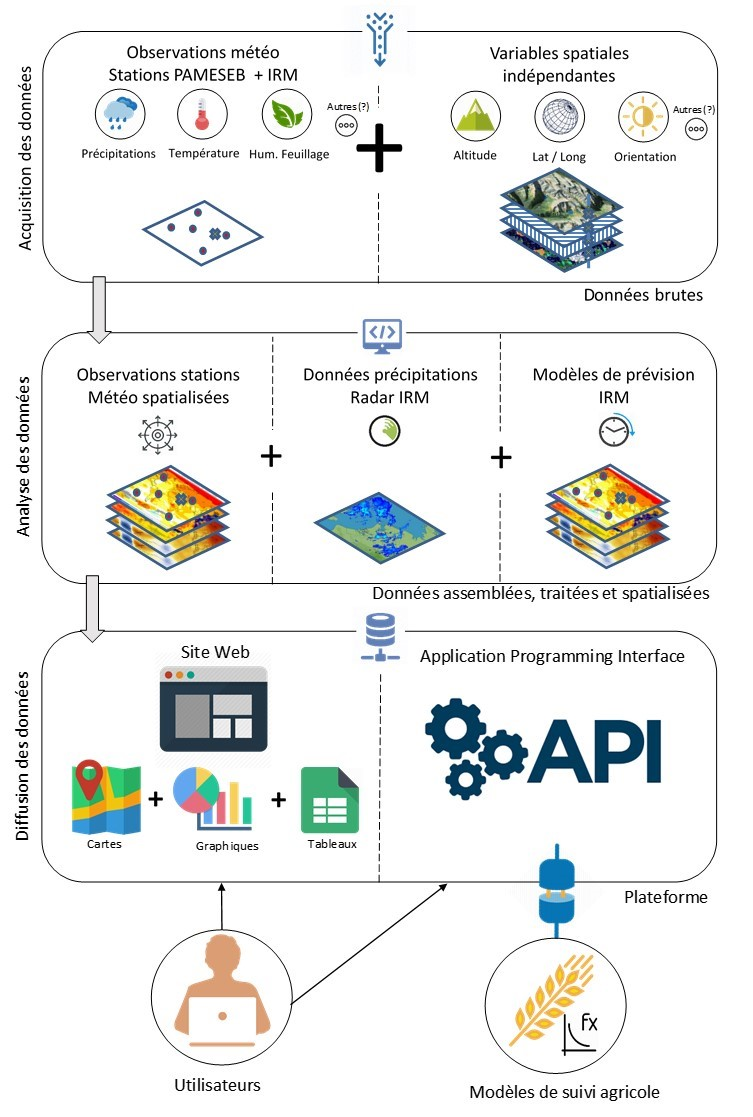
\includegraphics[width=0.65\linewidth]{figure/agromet} 

}

\caption{First draft of the functional architecture of the platform}\label{fig:agromet}
\end{figure}
Meteorological data wanted to be predict are :
\begin{itemize}
\tightlist
\item
  Temperature (1.5 meters above the ground)
\item
  Relative humidity (1.5 meters above the ground)
\item
  Leaves wetness
\item
  Rainfall will be spatialized from RMI rain radar data.
\end{itemize}
To predict these variables, known data are used :
\begin{itemize}
\tightlist
\item
  Digital elevation model and its derivatives like aspect and slope
\item
  Solar irradiance
\item
  Other variables discussed to improve the prediction : distance to sea,
  CORINE land cover\ldots{}
\end{itemize}
The Figure \ref{fig:agromet} shows the architecture of the future
platform and steps before data diffusion.

\subsection{Importance of the internship for the
project}\label{importance-of-the-internship-for-the-project}

To predict meteorological variables, several statistical method will be
tested. The identified methods at this time are multiple linear
regression, ANN and several kriging methods.

Two objectives were clearly defined for my internship. I operated in the
data acquisition and data analysis steps with the aim of predicting
\textbf{temperature} using \textbf{Multiple linear Regression}.

First, I have collected data which can be explanatory variables for
temperature and organised them to be integrated in the analysis and
benchmark.

Then, I ran a benchmark experiment where different desired regression
learning algorithms are applied to various regression tasks
(i.e.~datasets with different combinations of explanatory variables and
the target weather parameter) with the aim to compare and rank the
combinations of algorithm and used explanatory variables using a cross
validation resampling strategy that provides the desired performance
metrics. And then, I aggregated, by calculating the mean, all the hourly
performance measures to choose the method that globally performs the
best. For each desired hourly dataset, I applied the choosen method to
build a model to make spatial predictions. The predictions and their
uncertainty have been vizualized using maps. Finally, I had to make the
predictions available on the platform together with its uncertainty
indicator.

For a matter of time, this benchmark is run on two large years (from
2015-11-11 to 2018-06-30) because some data were not available before
this period.

\chapter{Working environment}\label{workenv}

\section{Applications and tools}\label{applications-and-tools}

Working in development field often imposes to be methodic. That's why
preparing the working environment is very important.

First, I have installed \textbf{Ubuntu GNOME}, a distribution of Linux
on my laptop. Indeed, this OS is prefered by developers and open-source
addicts thanks to the high contribution to improve distributions. Linux
distributions are safer than Windows due to that and it is very easy to
automatise a lot of commands. This installation was done thanks to a USB
drive with a boot of Ubuntu GNOME.

Once I had Ubuntu installed on my laptop, I used an \textbf{ANSIBLE
script} to install all the applications I need automatically. Moreover,
this script handles the updates of these applications. That is a very
useful way to earn some time.

Accessing to servers has to be secured. That's why every developer
should have a \textbf{SSH} key. This key or token is unique and enable
people to access to servers. It is useful to access to Git repositories
for example.

\textbf{GitHub} is a hosting service for version control. Its
utilisation is very common for developers because their codes are
online, the access is public and GitHub enable to handle versions of
files. It makes easier the collaborative work on a same code and enable
to use codes of other users.

For my internship, I need to work with my mentor to code. GitHub is the
best solution to that. I created a folder in my laptop to clone all the
repositories I need for my work. Then, I have a copy that I can modify
and I can send my modifications on GitHub. To clone these repositories,
my SSH key was useful.

The AGROMET project for whom I worked has an \textbf{API} to store
meteorological data from all the stations. An account has been created
for my internship. Then, I can get data from the API to test my codes.
These data have JSON or GeoJSON format, a open-standard file format
derived from JavaScript which is easy for machines to parse and generate
and easy to read and write for humans.

\textbf{Docker} is a software for containerize platforms. This container
approach has many advantages compares to the use of virtual machines :
lightweight, quick and modular.

There are two main reasons to use R in conjunction with Docker. First,
it allows you to quickly and easily share your work whatever the OS and
R configuration of your collaborators. Second, it allows you to work in
an isolated environment. This means that you will never pollute your OS
and e.g.~run in time-consuming re-installation procedures due to broken
configuration. In case of OS crash, simply relaunch your Docker R
container with a single command and you are ready to work.

\section{Reproducible science}\label{reproducible-science}

The AGROMET project is a public one. That means that the CRA-W and all
people involved have to be transparent about the work and the results.
That will give to the project more credibility and more reliability.

Transparency is promoted thanks to open science. That means the content
and the results of the project will be accessible to others. Indeed,
transparency is superior to trust and is an ideal (Munafo, 2017).

In the case of the project, development represents its major part.
Today, open science is widely used and tools have been developed for
that. That insures to all codes written for the project to be available.
As a consequence, anyone will be able to check the code and inspect it.
Then, some people can improve codes and increase efficiency of work.

Moreover, this transparency insures that the models built will be
completely explicit for people who will use them. That is a proof of the
quality of models.

\chapter{Data acquisition and preparation}\label{data-acq}

Variables have to be identified to build models. To do that, we need
response variables, i.e.~variables to predict, and explanatory
variables, i.e.~variables on which response variables depend.

\section{Interest variables}\label{interest-variables}

The AGROMET project will provide information about weather parameters
which are important for some crop diseases. These parameters are
temperature, relative humidity, leaves wetness and rainfall. The last
one is retrieved from a Dutch company. The others are measured by
weather stations from PAMESEB network, data are stored on an API. This
API is an intermediary software where we can make requests to get some
data. Data extracted from the API need to be transformed to be more
manipulable. Functions were wrote to transform these data. For example,
convert measures from character to numeric.

\section{Explanatory variables}\label{explanatory-variables}

A little reminder : I will use multiple linear regression. That means I
want to find an equation where a response variable can be modeled from
two or more variables. The equation will have the form :
\(Y = b_0 + b_1.X_1 + b_2.X_2 + ... + b_n.X_n\) where \(Y\) is the
response variable and \(X_n\) your \(n\) explanatory variables related
to their estimated parameter \(b_n\).

These explanatory variables have been identified from academic papers
(Zeuner 2007, Janssen 2011). Two types of explanatory variables can be
discriminate : static variables and dynamic variables.

\subsection{Static variables}\label{static-variables}

\subsubsection{Land cover}\label{land-cover}

All PAMESEB weather stations are sited in agricultural or herbaceous
areas. That is a way to reduce errors about measures. However, the
environment of each station can be different and can have an impact on
measures. For example, a station could have a different behaviour if a
forest is near its area or if an artificial surface (road, construction)
is near it.

CORINE land cover is an inventory updated every 6 years by
\textbf{Copernicus}, the European Union's Earth Observation Programme.
These data can also be found on the \textbf{Belgian geo-portal}. CORINE
Land Cover has been already used to make a spatial interpolation of air
pollution (Janssen \emph{et al.} 2011).

CORINE Land Cover is divided in 47 different land covers. 26 of them are
in Wallonia. However, 26 land covers is too much to be integrated as
explanatory variables. These land covers have been grouped in 5 classes
we juged relevant :
\begin{itemize}
\item
  \textbf{Agricultural areas} : areas where crops can be tall
\item
  \textbf{Herbaceous vegetation} : cleared areas like pastures and
  grasslands
\item
  \textbf{Artificial areas} : roads, rails and constructions where
  anthropogenic material can impact temperature
\item
  \textbf{Forest} : large areas providing shadow and cold
\item
  \textbf{Water bodies} : areas like river, lake, wetlands and bogs.
  Finally, this class has been removed because of the fact that no
  stations are located near a water body
\end{itemize}
After a long data preparation with transformation of CRS from WGS84 to
Belgian Lambert 2008 and conversion in different forms of Spatial
objects (Vector and Raster), data were completely manageable.

Finally, data are recovered at stations positions with buffers. These
buffers have a radius of 100 meters for physical stations and 500 meters
for virtual stations (because each station covers 1 km²). The Table
\ref{tab:clcperc} below shows the structure of the data frame where each
station identified by an ID has the percentage of cover for each class.
\begin{table}

\caption{\label{tab:clcperc}Distribution of land covers around physical stations}
\centering
\begin{tabular}[t]{rrrrr}
\toprule
\textbf{sid} & \textbf{crops} & \textbf{artificial} & \textbf{forest} & \textbf{herbaceous}\\
\midrule
1 & 63.85818 & 4.265755 & 0.00000 & 31.83038\\
4 & 64.11932 & 35.834990 & 0.00000 & 0.00000\\
7 & 75.28137 & 0.000000 & 0.00000 & 24.67295\\
9 & 99.95431 & 0.000000 & 0.00000 & 0.00000\\
10 & 69.91902 & 0.000000 & 30.03530 & 0.00000\\
13 & 89.50912 & 0.000000 & 10.44519 & 0.00000\\
\bottomrule
\end{tabular}
\end{table}
Buffers of 500 meters radius and grid cells of 1km² were compared but
buffers were chosen because they have more relevance when they are
compared to physical stations where only buffers were computed.

\subsubsection{Digital Terrain Model}\label{digital-terrain-model}

In the same way as land cover, the terrain model could have an impact on
temperature of the environment. These variables have been integrated in
the models made by Zeuner \emph{et al.} (2007) and the relevance has
been demonstrated several times.

Elevation data have been recovered for Wallonia from \textbf{NASA's
SRTM} providing a high-resolution (90 meters) topographic data. Then,
slope, aspect and roughess of terrain have been calculated with spatial
libraries from R. These data are very large and data processing is very
long because resolution is high.

\subsection{Dynamic Variables}\label{dynamic-variables}

\subsubsection{Solar irradiance}\label{solar-irradiance}

In the same way as temperature is a dynamic variable, explanatory
variables can be dynamic. In the case of temperature, we can be
interested in solar irradiance. Indeed, solar irradiance has an impact
on climate changes (Dewitte \emph{et al.} 2004).

Data are recovered from \textbf{EUMETSAT}, the European Organisation for
the Exploitation of Meteorological Satellites. They are produced every
30 minutes and expressed in W/m². These data are aggregated in hourly
data and they are stored on a API of AGROMET.

Data are available from 2015-11-11. As a consequence, we can not build
models from data before this date.

In parallel with that, PAMESEB stations also measure solar irradiance.
But only 27 stations are useable.

\subsubsection{Temperature forecasts}\label{temperature-forecasts}

The AGROMET project is supported by RMI, the Belgian equivalent of Météo
France. As a partner, RMI will provide temperature forecasts based on
their own algorithms. These data will be integrated as explanatory
variables to build models.

At the time of my internship, these data were not available.

\section{Data organisation}\label{data-organisation}

Once all the data are available, an important task is to organize them
to realise the modeling. This organisation needs to respond to a
methodic approach. Indeed, to reduce computation time, structure of data
have to be optimised.

The objective is to build models for each hour and compute its related
error.

The first step consists of grouping data. Static and dynamic variables
are grouped in a data frame. Then, to reduce time computation and to
prepare the integration of the data frame for the modeling, there is a
way to nest data frames with the library purrr. In this way, it is
possible to have one single row for each hour but every row contains
data frames inside. The Figure \ref{fig:nested} shows how it looks. This
nested data frame is a efficient way to manipulate many sub-tables at
once.
\begin{figure}

{\centering 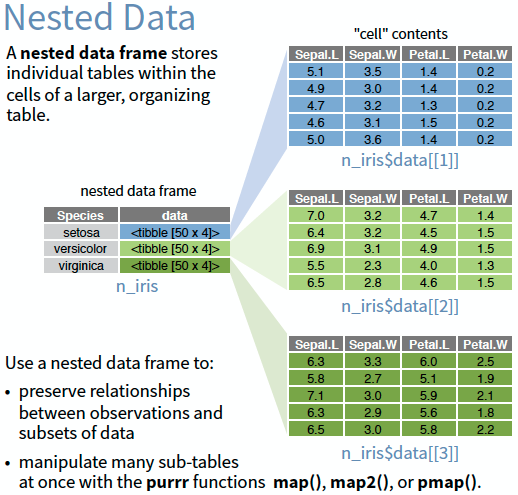
\includegraphics[width=0.5\linewidth]{figure/purrr_nest} 

}

\caption{Structure of a nested data frame}\label{fig:nested}
\end{figure}
In the case of the project, the nested data frame contains one row for
each hour which has a data frame containing data from each station at
this time. In the Table \ref{tab:ndf}, there is a preview of the data
frame contained into each row.
\begin{table}

\caption{\label{tab:ndf}Example of nested data frame in a row corresponding to 2016-05-19 15:00:00}
\centering
\resizebox{\linewidth}{!}{
\begin{tabular}[t]{r|r|r|r|r|r|r|r|r|r|r|r}
\hline
\textbf{altitude} & \textbf{slope} & \textbf{aspect} & \textbf{roughness} & \textbf{crops} & \textbf{artificial} & \textbf{forest} & \textbf{herbaceous} & \textbf{ens} & \textbf{tsa} & \textbf{X} & \textbf{Y}\\
\hline
473.6300 & 3.392046 & 211.6529 & 12.917668 & 63.85818 & 4.265755 & 0.00000 & 31.83038 & 348 & 12.4 & 721240.2 & 568849.6\\
\hline
345.7340 & 1.908891 & 162.7127 & 9.446796 & 64.11932 & 35.834990 & 0.00000 & 0.00000 & 389 & 12.8 & 714221.2 & 543453.8\\
\hline
348.8835 & 2.611751 & 165.0716 & 10.269126 & 75.28137 & 0.000000 & 0.00000 & 24.67295 & 779 & 14.1 & 750500.7 & 550825.6\\
\hline
497.7260 & 1.823958 & 137.0710 & 8.165029 & 99.95431 & 0.000000 & 0.00000 & 0.00000 & 916 & 13.5 & 753130.6 & 581716.9\\
\hline
389.9188 & 6.510637 & 310.6517 & 22.573696 & 69.91902 & 0.000000 & 30.03530 & 0.00000 & 916 & 14.9 & 734687.9 & 580969.6\\
\hline
259.7389 & 1.669001 & 288.5355 & 6.330072 & 89.50912 & 0.000000 & 10.44519 & 0.00000 & 774 & 15.2 & 641664.8 & 588814.6\\
\hline
\end{tabular}}
\end{table}
\chapter{Modeling with machine learning methods}\label{model}

Once the dataset is ready, the next step is to model predictions of
temperature. To do that, machine learning is used through R.

\section{Principle of machine
learning}\label{principle-of-machine-learning}

\subsection{Definition}\label{definition}

Machine learning is the idea that there are generic algorithms that can
tell you something interesting about a set of data without you having to
write any custom code specific to the problem. Instead of writing code,
you feed data to the generic algorithm and it builds its own logic based
on the data. In other words, Machine learning is a subset of deep
learning or Artificial Intelligence that provides an ability to
``learn'' with data.

There are 2 types of machine learning : supervised and unsupervised
learning.

\subsection{Supervised Machine
Learning}\label{supervised-machine-learning}

In practice, most of machine learning uses supervised learning.

From \emph{machinelearningmastery.com} :
\begin{quote}
Supervised learning is where you have input variables (x) and an output
variable (Y) and you use an algorithm to learn the mapping function from
the input to the output : Y = f(X). The goal is to approximate the
mapping function so well that when you have new input data (x), you can
predict the output variables (Y) for that data. It is called supervised
learning because the process of an algorithm learning from the training
dataset can be thought of as a teacher supervising the learning process
\end{quote}
In this learning, the algorithm tries to learn from examples we give to
it and then it returns a model of prediction. Classification and
regression are supervised machine learning.

This is the case of the AGROMET project where regression models are
used.

\subsection{Unsupervised machine
learning}\label{unsupervised-machine-learning}

Although that is not the subject, unsupervised learning consists in
algorithms which have to find themselves interesting structures in the
data. It differs from supervised learning because correct answers are
not given to the machine and it has to find answers itself. Association
and clustering are unsupervised machine learning.

For example, take 400 pictures of cats and 400 of dogs. While supervised
learning will give these pictures with the answer to the machine to make
it to find a way to discriminate cats and dogs, unsupervised learning
will give only the pictures and the machine will have to find itself
differences between cats and dogs separating them in two groups.
Obviously, the machine will not know that one group is corresponding to
cat and the other to dog because we did not labelled them but the
machine will be able to distinguish them like two separate entities.

\section{Machine learning approach in the AGROMET
project}\label{machine-learning-approach-in-the-agromet-project}

The objective is to predict weather parameters (temperature, relative
humidity, leaves wetness). We use data from meteorological stations and
from other sources like EUMETSAT for solar irradiance and COPERNICUS for
land cover.

Here is our approach :

We choose a weather parameter to predict, temperature for example. It is
our \textbf{target}.

Then, we define our \textbf{explanatory variables}, i.e.~the parameters
we want to build our model. These variables are our \textbf{task} and it
contains target data.

In our case, we will use several statistical methods to build our model
like kriging, multiple linear regression model or neural networks. Those
which are chosen to build a model are called \textbf{learners} and will
be compared.

To measure performance of our predictions, we need to use a
\textbf{cross-validation resampling strategy}. Several methods exist but
we will use the Leave-One-Out cross-validation method. It consists to
establish model based on every samples except one which will be the
sample where the model is tested to compute the error and then doing it
again as many times as the number of samples. The error measured for our
models will be the RMSE and MAE.

The entire methodology is detailed in the \emph{Appendix A}.

\section{Machine Learning in R}\label{machine-learning-in-r}

All of our work is done on RStudio. It is a very powerful open-source
software for R. Moreover, a R package which provides the infrastructure
to run machine learning is available. This package \textbf{mlr} is very
complete to build models, make predictions and evaluate performances.

Machine learning in R offers a common and simplified interface for all
statistical methods implemented in the package.

With this package, run a benchmark with several statistical methods can
be done on data from a period. This benchmark returns a lot of
informations.

It is possible to compare statistical methods through measures of error
like RMSE or MAE. Comparing several combinations of explanatory
variables is also possible.

\chapter{Results and discussion}\label{results}

\section{Benchmark}\label{benchmark}

\subsection{Methodology}\label{methodology}

To realize the benchmark, data from 2015-11-11 00:00:00 to 2018-06-30
00:00:00 were used. The objective is to run a benchmark on 5 years of
data but at this moment, solar irradiance data from EUMETSAT were not
available before this date. Here, the dataset has 23089 hours.

The learners were defined with filter methods, i.e.~the same statistical
method was applied to different combinations of explanatory variables.
For my internship, I only used \textbf{Multiple Linear Regression}.

The Table \ref{tab:explvar} shows the different combinations used and
compared.

Every computation is done for each hour. As a consequence, the
combination of explanatory variables is not unique for each hour but
depends on a condition checked every time.

Performances were measured with a Leave-One-Out cross-validation
resampling strategy.

The benchmark took about 30 hours, i.e.~3 hours per method. Computations
are very long and results are very large. Each method represents more
than 1 Gigabyte of data.
\begin{longtable}[]{@{}clc@{}}
\toprule
\begin{minipage}[b]{0.18\columnwidth}\centering\strut
Statistical Method\strut
\end{minipage} & \begin{minipage}[b]{0.21\columnwidth}\raggedright\strut
ID\strut
\end{minipage} & \begin{minipage}[b]{0.52\columnwidth}\centering\strut
Explanatory Variables\strut
\end{minipage}\tabularnewline
\midrule
\endhead
\begin{minipage}[t]{0.18\columnwidth}\centering\strut
Multiple Linear Regression\strut
\end{minipage} & \begin{minipage}[t]{0.21\columnwidth}\raggedright\strut
\emph{lm.Long.Lat}\strut
\end{minipage} & \begin{minipage}[t]{0.52\columnwidth}\centering\strut
Longitude \& Latitude\strut
\end{minipage}\tabularnewline
\begin{minipage}[t]{0.18\columnwidth}\centering\strut
Multiple Linear Regression\strut
\end{minipage} & \begin{minipage}[t]{0.21\columnwidth}\raggedright\strut
\emph{lm.Long.Lat.Elev}\strut
\end{minipage} & \begin{minipage}[t]{0.52\columnwidth}\centering\strut
Longitude \& Latitude \& Elevation\strut
\end{minipage}\tabularnewline
\begin{minipage}[t]{0.18\columnwidth}\centering\strut
Multiple Linear Regression\strut
\end{minipage} & \begin{minipage}[t]{0.21\columnwidth}\raggedright\strut
\emph{lm.SolIrr+1bestVar}\strut
\end{minipage} & \begin{minipage}[t]{0.52\columnwidth}\centering\strut
Solar Irradiance \& best variable based on an hourly linear correlation
computation\strut
\end{minipage}\tabularnewline
\begin{minipage}[t]{0.18\columnwidth}\centering\strut
Multiple Linear Regression\strut
\end{minipage} & \begin{minipage}[t]{0.21\columnwidth}\raggedright\strut
\emph{lm.SolIrr+2bestsVar}\strut
\end{minipage} & \begin{minipage}[t]{0.52\columnwidth}\centering\strut
Solar Irradiance \& 2 bests variables based on an hourly linear
correlation computation\strut
\end{minipage}\tabularnewline
\begin{minipage}[t]{0.18\columnwidth}\centering\strut
Multiple Linear Regression\strut
\end{minipage} & \begin{minipage}[t]{0.21\columnwidth}\raggedright\strut
\emph{lm.SolIrr+3bestsVar}\strut
\end{minipage} & \begin{minipage}[t]{0.52\columnwidth}\centering\strut
Solar Irradiance \& 3 bests variables based on an hourly linear
correlation computation\strut
\end{minipage}\tabularnewline
\begin{minipage}[t]{0.18\columnwidth}\centering\strut
Multiple Linear Regression\strut
\end{minipage} & \begin{minipage}[t]{0.21\columnwidth}\raggedright\strut
\emph{lm.2bestsVar}\strut
\end{minipage} & \begin{minipage}[t]{0.52\columnwidth}\centering\strut
2 bests variables based on linear correlation computation for every
hour\strut
\end{minipage}\tabularnewline
\begin{minipage}[t]{0.18\columnwidth}\centering\strut
Multiple Linear Regression\strut
\end{minipage} & \begin{minipage}[t]{0.21\columnwidth}\raggedright\strut
\emph{lm.3bestsVar}\strut
\end{minipage} & \begin{minipage}[t]{0.52\columnwidth}\centering\strut
3 bests variables based on linear correlation computation for every
hour\strut
\end{minipage}\tabularnewline
\begin{minipage}[t]{0.18\columnwidth}\centering\strut
Multiple Linear Regression\strut
\end{minipage} & \begin{minipage}[t]{0.21\columnwidth}\raggedright\strut
\emph{lm.4bestsVar}\strut
\end{minipage} & \begin{minipage}[t]{0.52\columnwidth}\centering\strut
4 bests variables based on linear correlation computation for every
hour\strut
\end{minipage}\tabularnewline
\begin{minipage}[t]{0.18\columnwidth}\centering\strut
Multiple Linear Regression\strut
\end{minipage} & \begin{minipage}[t]{0.21\columnwidth}\raggedright\strut
\emph{lm.Vars.r\textgreater{}0,5}\strut
\end{minipage} & \begin{minipage}[t]{0.52\columnwidth}\centering\strut
Variables with a linear correlation greater than 0.5\strut
\end{minipage}\tabularnewline
\begin{minipage}[t]{0.18\columnwidth}\centering\strut
Multiple Linear Regression\strut
\end{minipage} & \begin{minipage}[t]{0.21\columnwidth}\raggedright\strut
\emph{lm.Vars.r\textgreater{}0,3}\strut
\end{minipage} & \begin{minipage}[t]{0.52\columnwidth}\centering\strut
Variables with a linear correlation greater than 0.3\strut
\end{minipage}\tabularnewline
\bottomrule
\end{longtable}
Table : \label{tab:explvar} Combinations of explanatory variables used

\subsection{Comparison of methods}\label{comparison-of-methods}

Once benchmark results are available, comparison of methods is possible.
This comparison is based on the error of measures. In our case, RMSE and
MAE were computed.

MAE measures the average magnitude of the errors in a set of
predictions, without considering their direction. It is the average over
the test sample of the absolute differences between prediction and
actual observation where all individual differences have equal weight.
\[
MAE = \frac{1}{n} \sum_{i=1}^{n}{ \lvert y_{j} - \widehat{y}_{j} \rvert}
\]

RMSE is a quadratic scoring rule that also measures the average
magnitude of the error. It is the square root of the average of squared
differences between prediction and actual observation.

\[
RMSE = \sqrt{\frac{1}{n} \sum_{i=1}^{n}{( y_{j} - \widehat{y}_{j} )^2}}
\]

They both express average model prediction error in units of the
variable of interest. Both metrics can range from 0 to \(\infty\) and
are indifferent to the direction of errors. They are negatively-oriented
scores, which means lower values are better.

Since the errors are squared before they are averaged, the RMSE gives a
relatively high weight to large errors. This means the RMSE is more
useful because large errors are particularly undesirable in the project.
(Chai, 2014)

From the 10 methods compared, MAE and RMSE are computed and compared.
The results are shown in the Figure \ref{fig:meanerror}. In this case,
they both have the same behaviour. Multiple linear regression using
coordinates to build models has a large error, the model is too
simplified. Multiple linear regression using explanatory variables whose
their linear correlations with temperature is greater than 0.3 has an
error larger than the other methods too, this filter method is too
flexible to return a valid model. A few methods have a similar error. In
particular, that is the case when too many variables are chosen to build
models.

On the three best methods, one is better than the others. That is the
model built from an equation using longitude, latitude and altitude as
explanatory variables. Tests realized on two months of data have already
shown that altitude is a powerful explanatory variable. The two other
methods are based on the computation of the linear correlations with
temperature, with or without solar irradiance as mandatory variable have
a similar error. However, they are more interesting because the equation
is dynamic throughout hours and, in this way, the model is adapted to
the evaluated hour.
\begin{figure}

{\centering 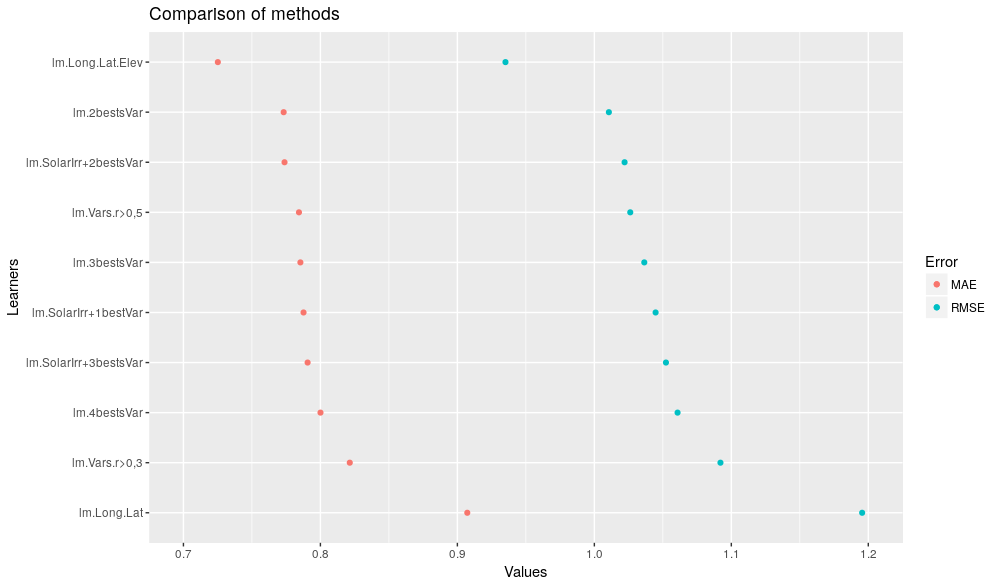
\includegraphics[width=1\linewidth]{figure/meanerror} 

}

\caption{Errors (RMSE and MAE) of methods}\label{fig:meanerror}
\end{figure}
Errors are between 0.72 and 0.91 for MAE and between 0.93 and 1.20 for
RMSE. These errors should be near zero. Both of MAE and RMSE are
expressed in degrees such as temperature. An error of 1 degree is
relatively important and has to be taken into consideration.

Performances of methods can be compared computing their rank for each
hour. The Figure \ref{fig:barchart} compares five of the bests methods :
\begin{itemize}
\tightlist
\item
  the 2 variables with the best linear correlation with temperature
\item
  longitude, latitude and elevation
\item
  solar irradiance and the 2 variables with the best linear correlation
  with temperature
\end{itemize}
This barchart corroborates the precedent graph. The method based on
coordinates and elevation is widely better than the two others which are
more similar but with a relevant difference.
\begin{figure}

{\centering 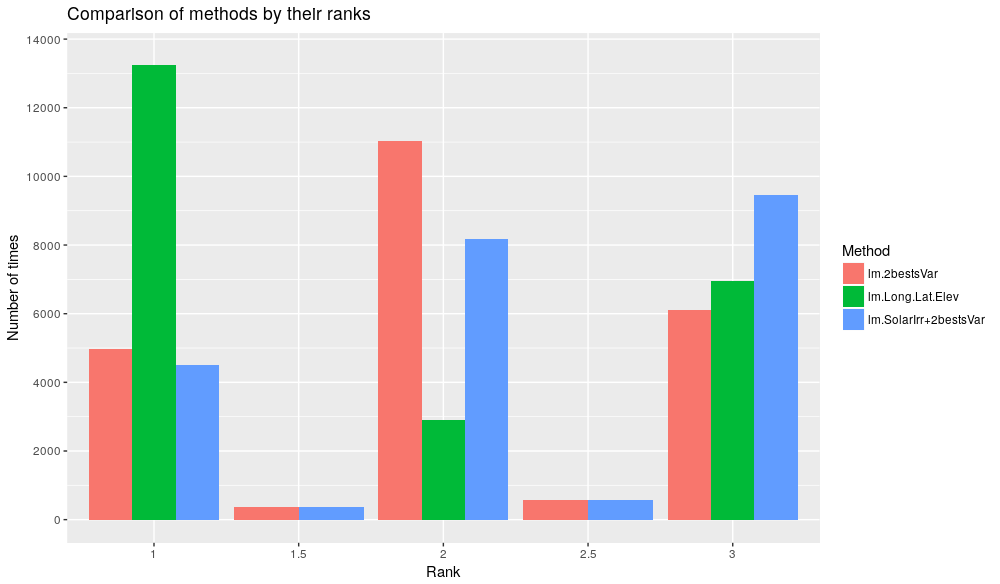
\includegraphics[width=1\linewidth]{figure/barchart} 

}

\caption{Comparison of methods by rank}\label{fig:barchart}
\end{figure}
For each hour, the equation of the model is computed. They can be
extracted from the benchmark. The Table \ref{tab:models} shows the
structure of the equations in the case where explanatory variables can
be different from one hour to another (lm.2bestsVar). The table also
shows what are the bests variables and display the related error.
\begin{table}

\caption{\label{tab:models}Models with their equations}
\centering
\resizebox{\linewidth}{!}{
\begin{tabular}[t]{l|l|l|l|l|r|r}
\hline
\textbf{ } & \textbf{Datetime} & \textbf{Equation} & \textbf{BestVar1} & \textbf{BestVar2} & \textbf{RMSE} & \textbf{MAE}\\
\hline
16135 & 2017-09-13 06:00:00 & T = 14.656695 + -0.008887.altitude + 1e-06.X & altitude & X & 0.5674956 & 0.4107285\\
\hline
16136 & 2017-09-13 07:00:00 & T = 14.722147 + -0.00574.altitude + 0.012719.ens & altitude & ens & 0.6122121 & 0.4529545\\
\hline
16137 & 2017-09-13 08:00:00 & T = 15.676696 + -0.004304.altitude + -0.011732.herbaceous & altitude & herbaceous & 0.9375293 & 0.7287999\\
\hline
16138 & 2017-09-13 09:00:00 & T = 13.701668 + -0.012835.herbaceous + 0.00415.ens & herbaceous & ens & 1.2198397 & 0.9671947\\
\hline
16139 & 2017-09-13 10:00:00 & T = 14.987154 + -0.001473.altitude + -0.009431.herbaceous & altitude & herbaceous & 1.0206276 & 0.8224733\\
\hline
16140 & 2017-09-13 11:00:00 & T = 14.131936 + -0.003737.altitude + 0.005707.ens & altitude & ens & 0.8312792 & 0.5979420\\
\hline
16141 & 2017-09-13 12:00:00 & T = 11.852128 + -0.002653.altitude + 0.012421.ens & altitude & ens & 0.9727891 & 0.7488237\\
\hline
16142 & 2017-09-13 13:00:00 & T = 22.557946 + 0.003638.ens + -1.4e-05.Y & ens & Y & 1.2605875 & 0.9444467\\
\hline
16143 & 2017-09-13 14:00:00 & T = 15.441184 + 0.000484.altitude + -0.015099.herbaceous & altitude & herbaceous & 1.0796645 & 0.8760026\\
\hline
16144 & 2017-09-13 15:00:00 & T = 10.730857 + -0.003947.altitude + 9e-06.Y & altitude & Y & 0.9526830 & 0.7777128\\
\hline
\end{tabular}}
\end{table}
\subsection{Vizualisation}\label{vizualisation}

These models can be observed on maps. For that purpose, functions
building maps have been made with ggplot2 library from R for static maps
and leaflet library for interactive maps.

Models built from physical stations data are applied to the 1 km² grid
cells. Then, the temperature is mapped with a color palette similar to
the one of RMI. Class breaks are based on quantiles of temperature
values. Standard error is computed for each cell and it is shown on the
map with a white layer which has different levels of transparency
according to the error. A large standard error is related to an opacity
and vice-versa.

The Figure \ref{fig:map} shows an output for one hour based on the
method ::todo::. To build this map, some objects are needed : an object
containing data (temperature and standard error) for the grid and a
spatial vector object containing boundaries of Wallonia, but also the
name of the variable to display. Then, some conditions can be chosen,
like the display of the layer containing error, the display of the
legend for error, the way to build the legend and its classes. Some
arguments enable to customize the map with titles and comments. The
function is thus reusable for other usages. For example, the function
builds maps spatializing hydric deficit in Wallonia.

This figure shows the output based on a model depending on ::todo::, the
equation is the following one :

{[}

{]}

These maps show whether the models are relevant. The \emph{Appendix B}
shows maps made with all methods for one hour. These maps show
differences in the relevance of each model. For example, the model
depending on longitude and latitude is very simplistic compared to the
others. The other models are more similar but show that some of them are
more reliable because the error is smaller. The better model is the
second one on the first row. It is corresponding to the the model
depending on longitude, latitude and elevation. For this hour, the model
is the following : \[
T = -9.375042 + -0.010431 \times Elevation + 1.02e-05 \times Longitude + 1.59e-05 \times Latitude
\]

Longitude and latitude are expressed in meters because the CRS used is
Belgian Lambert 2008. That is why their coefficients are about 1e-05.
For information, values of the coordinates are about 6e06.

::todo:: interpretation

::todo:: add example equations models tab

\section{Discussion}\label{discussion}

As a reminder, the objective of the project is to provide weather
predictions. These predictions will feed decision support tools to
monitor crop diseases like potato late blight and to operate in fields
at the right times.

Results have some limits that have to be discussed. The first limit is
the period used to build models. Indeed, models were built with data
from 2 and a half years. This period could be too short to be relevant.
Moreover, this period is not necessarily representative of a mean
period. According to RMI, 2015, 2017 and 2018 are hot and dry years
compared to normal year, 2016 were a wet year. This is shown on the
Figure \ref{fig:rmi}.
\begin{figure}

{\centering 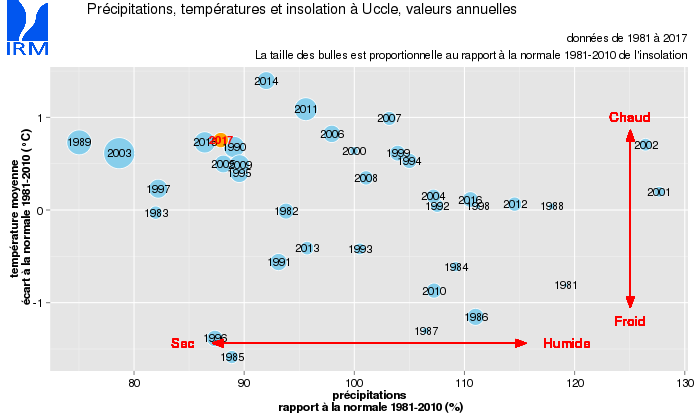
\includegraphics[width=400px,height=300px]{figure/rmi_climate_data} 

}

\caption{Precipitations, temperatures and insolation, annual values}\label{fig:rmi}
\end{figure}
Models were built with some explanatory variables but they may be
insufficient. Adding new variables like temperature predictions from RMI
could improve models. Only 27 stations are used to build these models,
adding RMI stations network could be a solution to improve models too.
However, weather stations from different networks have differences in
their measures, checking interoperability is very important for that and
making corrections is essential.

Multiple linear regression is the only statistical method used to build
models, but going forward, other methods will be compared like ANN and
different kriging methods. The major constraint will be time computation
which is relatively long. There is a lot of possible combinations of
explanatory variables to compare, choices must be done because of the
time computation. These choices sometimes can be subjective and not
based on scientific literature.

Beyond these limits, other points can be discussed. For example, solar
irradiance data are provided by EUMETSAT and by PAMESEB stations. These
data have to be compared because both sources are used. Data from
stations are used to build models, data from EUMETSAT for
spatialization. The comparison shows a correlation around 0.95. As a
consequence, there is nothing wrong with it.

With the aim to provide data for agronomic utilisation, there is an
interest to compare mean error observed in Wallonia and this error in
agricultural areas to be sure of the accuracy of predictions. ::todo::

Assuming that no other models will be better than those presented, there
will be a question of transparency for the project. Indeed, as a public
project within the scope of public agencies, the work that is done has
to be transparent. In that way, models will be clearly presented. If one
static model is chosen for predictions, this will be clear and
transparent. But if the chosen method is a dynamic one, using
computation every hour, the method used for each hour could be
different, and that will have to be mentioned.

\chapter*{Conclusion}\label{conclusion}
\addcontentsline{toc}{chapter}{Conclusion}

::todo::

\appendix

\chapter{Resources on AGROMET and my
work}\label{resources-on-agromet-and-my-work}
\begin{itemize}
\item
  Technical details about PAMESEB stations :
  \url{https://www.pameseb.be/meteo_intro/infos_techniques.html}
\item
  Spatialization methodology available here :
  \url{https://pokyah.github.io/agrometeor-methodo-spatial/assets/uml_images/spatialization-methodology.svg}
\item
  All my codes are available on my Github account :
  \url{https://github.com/ldavadan}
\item
  My personal blog, made with Blogdown : \url{ldavadan.github.io}
\item
  Contribution to ``Crop and Grassland conditions in early August''
  report :
  \url{http://www.cra.wallonie.be/fr/etat-des-cultures-et-des-prairies-en-ce-debut-du-mois-daout-2018}
\end{itemize}
\chapter{Outputs with different
methods}\label{outputs-with-different-methods}

Methods from left to right and top to bottom follow the order presented
in Table \ref{tab:explvar}. Models built for 2018-03-07 14:00:00.
\begin{center}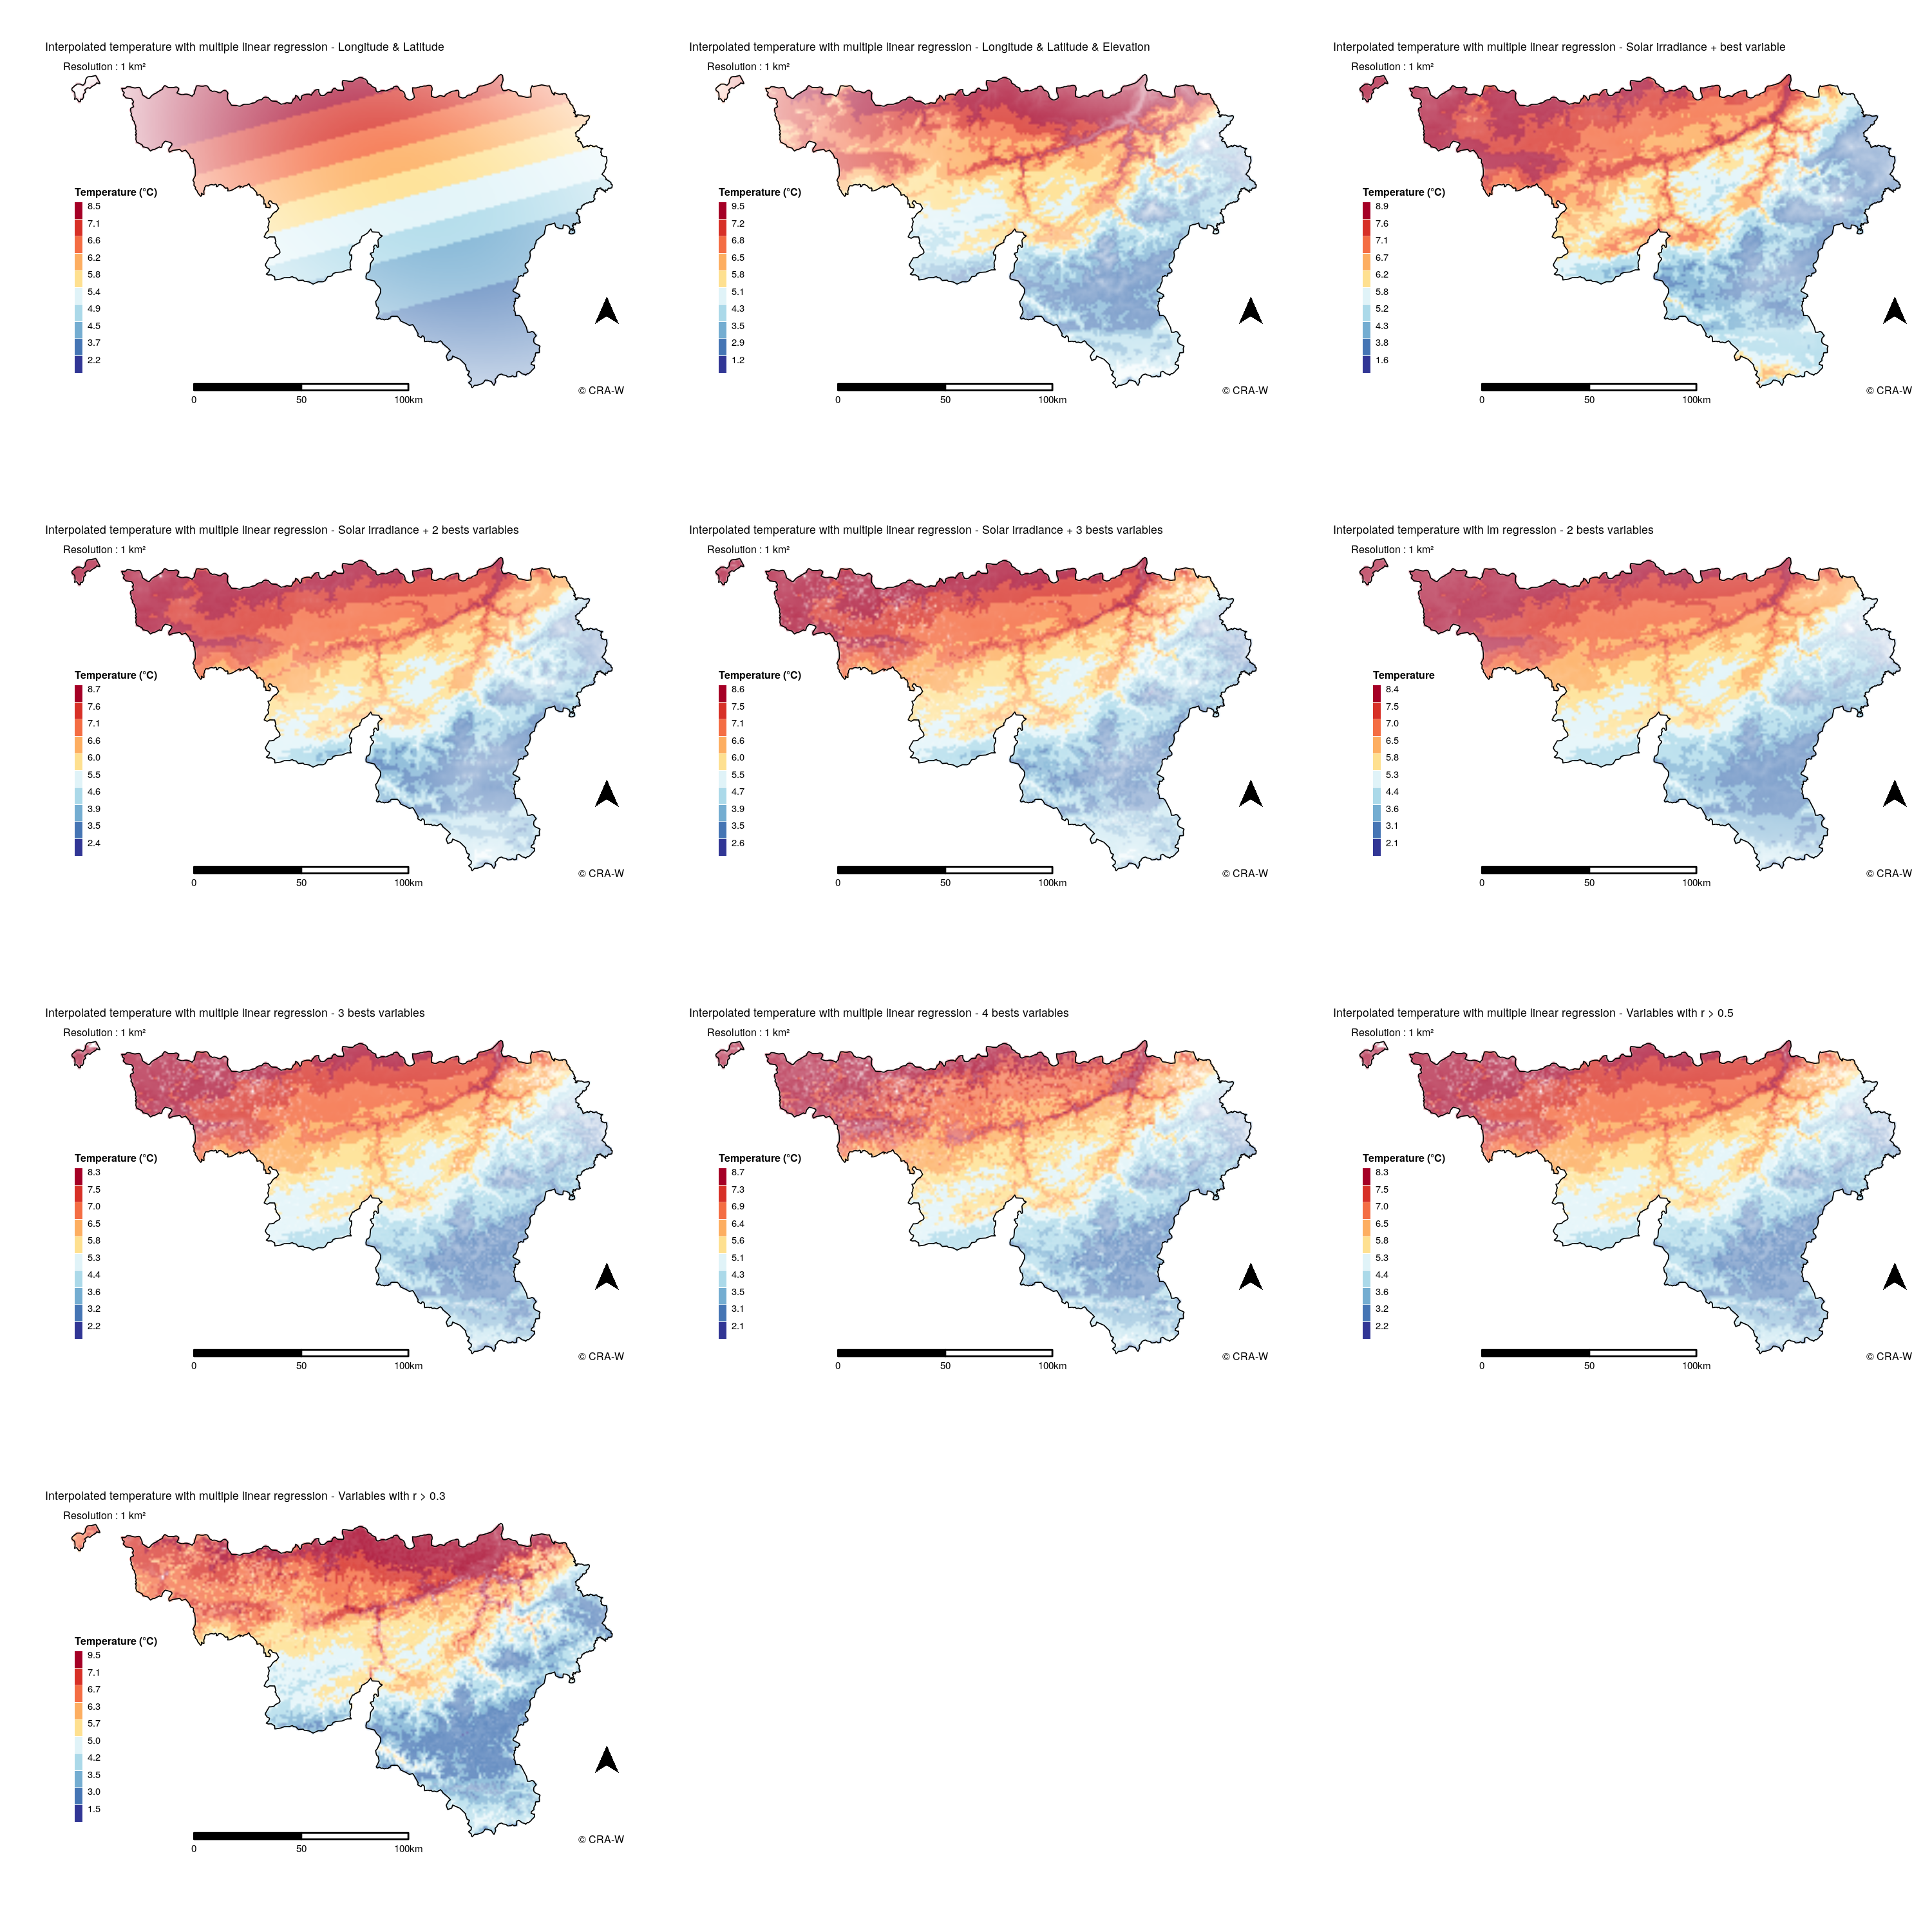
\includegraphics[width=1\linewidth]{figure/2018-03-07_14} \end{center}

\chapter{Additional resources}\label{additional-resources}
\begin{itemize}
\item
  Ubuntu GNOME : \url{https://ubuntugnome.org/}
\item
  ANSIBLE : \url{https://www.ansible.com/}
\item
  SSH : \url{https://www.ssh.com/}
\item
  GitHub : \url{https://github.com/}
\item
  API :
  \url{https://medium.freecodecamp.org/what-is-an-api-in-english-please-b880a3214a82}
\item
  Docker : \url{https://www.docker.com/what-docker}
\item
  Copernicus :
  \url{https://land.copernicus.eu/pan-european/corine-land-cover/view}
\item
  Belgian Geoportal :
  \url{https://www.geo.be/\#!/catalog/details/bcd19aa9-c320-4116-971b-6e4376137f13?l=en}
\item
  NASA's SRTM : \url{https://lta.cr.usgs.gov/SRTM}
\item
  EUMETSAT :
  \url{https://landsaf.ipma.pt/en/products/longwave-shortwave-radiation/dssf/}
\item
  Machine Learning Mastery Blog :
  \url{https://machinelearningmastery.com/supervised-and-unsupervised-machine-learning-algorithms/}
\item
  Machine Learning in R : \url{http://mlr-org.github.io/mlr/index.html}
\end{itemize}
\backmatter

\chapter*{References}\label{references}
\addcontentsline{toc}{chapter}{References}

\markboth{References}{References}

\noindent

\setlength{\parindent}{-0.20in} \setlength{\leftskip}{0.20in}
\setlength{\parskip}{8pt}

\hypertarget{refs}{}
\hypertarget{ref-chai2014}{}
Chai, T., \& Draxler, R. (2014). Root mean square error (rmse) or mean
absolute error (mae)? -- Arguments against avoiding rmse in the
literature. \emph{Geoscientific Model Development}, 1247--1250.

\hypertarget{ref-dewitte2004}{}
Dewitte, S., \& others. (2004). Measurement and uncertainty of the
long-term total solar irradiance trend. \emph{Solar Physics}, 209--216.

\hypertarget{ref-hooyberghs2006}{}
Hooyberghs, J., \& others. (2006). Spatial interpolation of ambient
ozone concentrations from sparse monitoring points in belgium. \emph{J.
Environ. Monit.}, 1129--1135.

\hypertarget{ref-janssen2008}{}
Janssen, S., \& others. (2008). Spatial interpolation of air pollution
measurements using corine land cover data. \emph{Atmospheric
Environment, Volume 42, Issue 20}, 4884--4903.

\hypertarget{ref-munafo2017}{}
Munafo, M., \& others. (2017). A manifesto for reproducible science.
\emph{Nature Human Behaviour Volume 1, Article Number: 0021}.

\hypertarget{ref-racca2011}{}
Racca, P., \& others. (2011). Decision support systems in agriculture :
Administration of meteorological data, use of geographic information
systems (gis) and validation methods in crop protection warning service.
\emph{Efficient Decision Support Systems - Practice and Challenges from
Current to Future}, 331--354.

\hypertarget{ref-zeuner2007}{}
Zeuner, T., \& Kleinhenz, B. (2007). Use of geographic information
systems in warning services for late blight. \emph{Bulletin OEPP/EPPO},
327--334.

% Index?

\end{document}
